\documentclass[UTF8]{ctexart}
\usepackage{ctex}
\usepackage{geometry}
\usepackage{enumitem}
\usepackage{indentfirst}
\usepackage{color}
\usepackage{fancyhdr}
\usepackage{amsmath}
\usepackage{graphicx}
\usepackage{amssymb}
\usepackage{tikz}
\usepackage{cases}
\usepackage{array}
\usepackage{mathrsfs}
\usepackage{pgfplots}
\usepackage{tkz-euclide}
\usepackage{ragged2e}
\pgfplotsset{compat=1.17}
\usetikzlibrary{arrows.meta, decorations.pathreplacing, calligraphy}

% 设置纸张和页边距——A4
\geometry{papersize={21cm,29.7cm}}
\geometry{left=3.18cm,right=3.18cm,top=2.54cm,bottom=2.54cm}

% 一级标题靠左
\CTEXsetup[format={\Large\bfseries}]{section}

% 去除页眉
\pagestyle{plain}

% 开始文档内容
\begin{document}

\title{信号与系统课程笔记:Lecture 15}
\author{授课教师:秦雨潇 \\
        笔记记录:李梦薇}
\date{2023 年 11 月 03 日(第九周,周五)}
\maketitle

\section{系统的数学表达}
\begin{enumerate}[label=(\arabic*),itemindent=0pt,labelindent=\parindent,labelwidth=2em,labelsep=5pt,leftmargin=*]
      \item $y=ax\quad\Longleftrightarrow\quad{Y=AX}$,$X=A^{-1}Y$
      \item $y=ax^2\quad$例如:CNN/DNN
\end{enumerate}\par
\subsection{电路}
\begin{figure}[h]
      \centering
      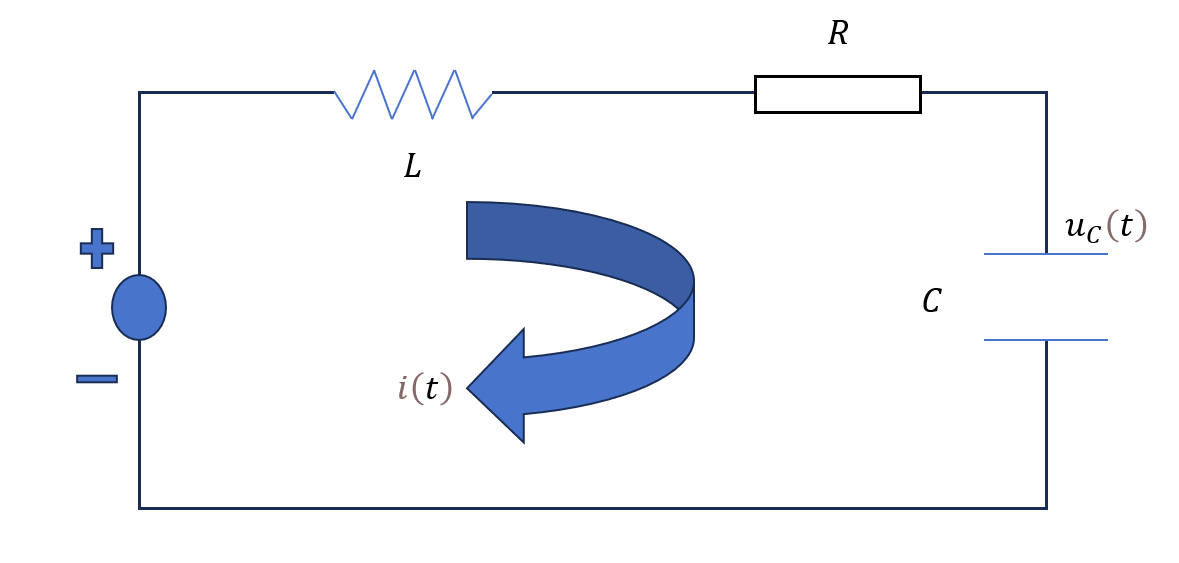
\includegraphics[scale=0.35]{电路.png}
\end{figure}
\begin{center}
      \begin{tabular}{ c c c }
            $U_S(t)$ & $\rightarrow$ & $U_C(t)$ \\
            输入 & $\quad$ & 输出 \\
            激励 & $\quad$ & 响应
      \end{tabular}
\end{center} \par
$U_S(t)=U_L(t)+U_R(t)+U_C(t)$ \par
其中,
$\left\{
      \begin{aligned}
            &U_R(t)=i(t)R \\
            &i(t)=\frac{{\rm{d}}}{{\rm{d}}t}U_C(t) \\
            &U_L(t)=\frac{{\rm{d}}}{{\rm{d}}t}i(t)
      \end{aligned}
\right.$ \par
$\Longrightarrow$
$\left\{
      \begin{aligned}
            &{U_S(t)}=U_C(t)+R\cdot{C}\cdot{U'_C(t)}+L\cdot{C}\cdot{U''_C(t)} \\
            &U_C(0)=U'_C(0)=0
      \end{aligned}
\right.$ \par
\newpage
\subsection{力学}
\begin{figure}[h]
      \centering
      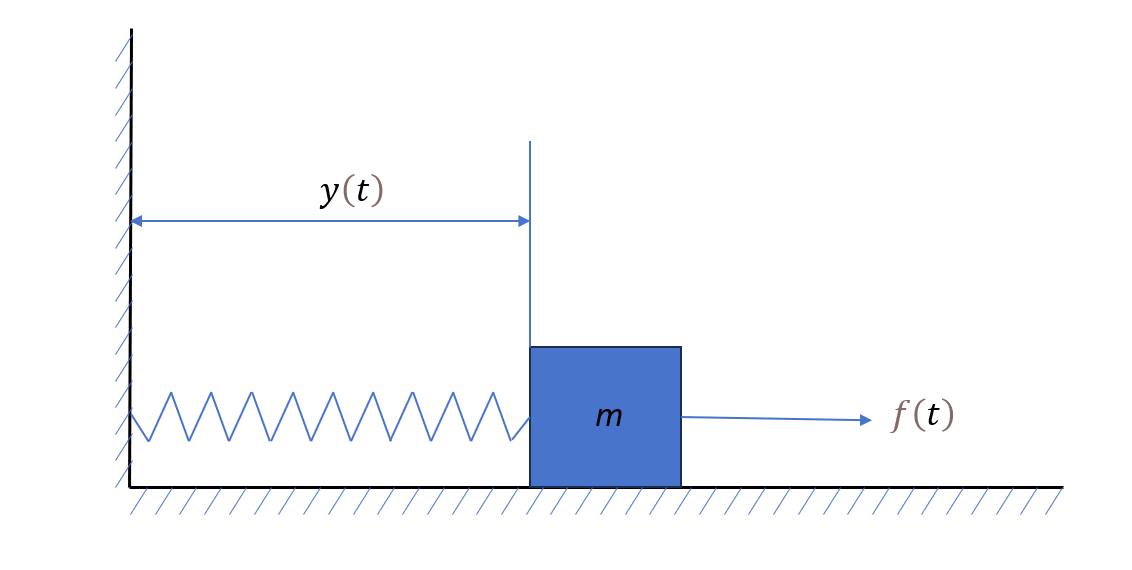
\includegraphics[scale=0.35]{力学.png}
\end{figure}
\begin{center}
      \begin{tabular}{ c c c }
            $f(t)$ & $\rightarrow$ & $y(t)$ \\
            输入 & $\quad$ & 输出
      \end{tabular}
\end{center} \par
$\left\{
      \begin{aligned}
            &F=ma=my''(t) \\
            &f(t)+ky(t)+\alpha{y'(t)}=F
      \end{aligned}
\right.$ \par
$\left\{
      \begin{aligned}
            &f(t)=my''(t)+\alpha{y'(t)}+ky(t) \\
            &y(0)=y'(0)=1
      \end{aligned}
\right.$ \par
\subsection{傅里叶铁棒实验(求解在某时刻铁棒在某处的温度)}
\begin{figure}[h]
      \centering
      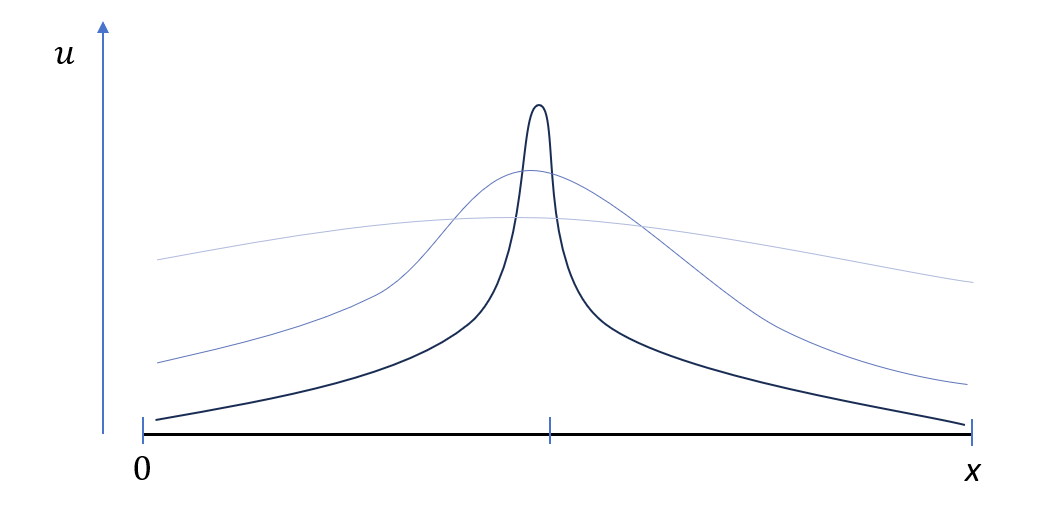
\includegraphics[scale=0.35]{傅里叶.png}
\end{figure}
$\left\{
      \begin{aligned}
            &\frac{\partial{u(x,t)}}{\partial{t}}=\alpha^2\frac{\partial^2{u(x,t)}}{\partial{x^2}} \\
            &u(x,0)\text{已知}
      \end{aligned}
\right.$ \par
$\left\{
      \begin{aligned}
            &\text{常微分方程(PDE)}\quad\rightarrow\quad\text{偏微分方程(ODE)} \\
            &\text{偏微分方程(ODE)}\quad\rightarrow\quad\text{线性方程(linear)}
      \end{aligned}
\right.$ \par
\subsection{结论}
许多系统($f(t)\rightarrow{y(t)}$/$y(t)=G(f(t))$)在数学上归纳为如下形式:\par
\noindent
\begin{flalign*}\hspace{2em}
      &\sum_{n=0}^{N}a_n\frac{{\rm{d}}^nf(t)}{{\rm{d}}t^n}=\sum_{m=0}^{M}b_m\frac{{\rm{d}}^my(t)}{{\rm{d}}t^m} &\\
\end{flalign*} \par

\section{响应的类型}
零输入响应+零状态响应=完全响应
\begin{enumerate}[label=(\arabic*),itemindent=0pt,labelindent=\parindent,labelwidth=2em,labelsep=5pt,leftmargin=*]
      \item 零状态响应:$y(t)=0\quad{t<0}$
      \item 零输入响应:$y(0)$可导,连续
\end{enumerate}\par
举例:卷积
\begin{tabular}{ c c c }
      $\int_{\mathbb{R}}f(\tau)\delta(t-\tau){\rm{d}}\tau$ & $\rightarrow$ & $\int_{\mathbb{R}}f(\tau)h(t-\tau){\rm{d}}\tau$ \\
      $f(t)$ & $\rightarrow$ & $f(t)*h(t)$ \\
\end{tabular}为零状态响应。

\section{基本信号的响应}
$e^{j\omega_0t}$基本信号$\quad\rightarrow\quad{h(t)}$系统$\quad\rightarrow\quad$?
\noindent
\begin{flalign*}\hspace{2em}
      e^{j\omega_0t}*h(t)&=\int_{\mathbb{R}}h(\tau)e^{j\omega_0t}\cdot{e^{-j\omega_0t}}{\rm{d}}\tau &\\
      &=e^{j\omega_0t}\int_{\mathbb{R}}h(\tau)\cdot{e^{-j\omega_0t}}{\rm{d}}\tau &\\
      &=e^{j\omega_0t}H(\omega_0)
\end{flalign*} \par

\end{document}